\chapter{Thực nghiệm và đánh giá}

\section{Bộ dữ liệu}
RACE (Reading Comprehension Dataset From Examinations) là một bộ dữ liệu quy mô lớn trong lĩnh vực xử lý ngôn ngữ tự nhiên. Khác với bộ dữ liệu SQuAD (chủ yếu dựa trên Wikipedia), RACE được xây dựng trực tiếp từ đề thi của các kỳ thi tiếng Anh thực tế dành cho học sinh trung học cơ sở và trung học phổ thông tại hệ thống giáo dục Trung Quốc.

Hai lý do chính nghiên cứu sử dụng RACE làm bộ dữ liệu đánh giá mô hình là:
Độ phức tạp và đa dạng ngữ nghĩa: Văn bản trong RACE thường bao trùm nhiều lĩnh vực trong đời sống: giáo dục, tin tức, văn hóa, chính trị, khoa học và các câu chuyện luân lý. Chính vì thế, đặc điểm dữ liệu và văn phong của văn bản trong RACE vô cùng sát với các tài liệu trong thực tế. Các văn bản trong RACE có độ dài tiêu chuẩn từ 300 đến 500 từ, độ dài này đủ lớn để chứa đựng lượng thông tin cho một bài kiểm tra: các chuỗi sự kiện phức tạp, luận điểm, nhưng vẫn đảm bảo không làm quá tải cửa sổ ngữ cảnh (context window) của các sLLM.

Chiều sâu logic và tính đa nghĩa của văn bản gốc: Không giống các văn bản bách khoa toàn thư chỉ liệt kê dữ liệu bề mặt, các văn bản của RACE được các chuyên gia giáo dục tuyển chọn chuyên biệt nhằm mục đích đánh giá nhận thức của người học. Cấu trúc của văn bản ẩn chứa nhiều tầng nghĩa, tích hợp các chuỗi nhân quả, thái độ ngầm định của tác giả và các mệnh đề gây nhiễu. Nếu nghiên cứu lựa chọn một bộ dữ liệu văn bản thiếu chiều sâu, các nỗ lực đánh giá LLM sinh câu hỏi tư duy cao đều sẽ thất bại.

% [NEW]
Bộ dữ liệu RACE bao gồm khoảng 28.000 đoạn văn và gần 100.000 câu hỏi trắc nghiệm, được chia thành hai tập con theo cấp độ: RACE-Middle (dành cho học sinh trung học cơ sở) và RACE-High (dành cho học sinh trung học phổ thông). Tập RACE-High chứa các đoạn văn có độ phức tạp cao hơn, đòi hỏi khả năng suy luận sâu hơn, do đó phù hợp hơn với mục tiêu đánh giá khả năng sinh câu hỏi đa cấp độ nhận thức của nghiên cứu này.

% [NEW]
Trong phạm vi thực nghiệm, nghiên cứu lấy mẫu ngẫu nhiên 100 đoạn văn từ tập RACE-High làm dữ liệu đầu vào cho toàn bộ các thí nghiệm sinh câu hỏi. Bảng~\ref{tab:race_stats} trình bày thống kê tổng quan về bộ dữ liệu RACE và mẫu được sử dụng.

% [NEW]
\begin{table}[htbp]
\centering
\label{tab:race_stats}
\begin{tabular}{lrrr}
\toprule
\textbf{Đặc điểm} & \textbf{RACE-Middle} & \textbf{RACE-High} & \textbf{Mẫu thực nghiệm} \\
\midrule
Số đoạn văn & $\sim$6.400 & $\sim$21.600 & 100 \\
Số câu hỏi & $\sim$25.400 & $\sim$72.000 & - \\
Nguồn gốc & Đề thi THCS & Đề thi THPT & Lấy mẫu từ RACE-High \\
Độ dài trung bình (từ) & 250-350 & 300-500 & 300-500 \\
\bottomrule
\end{tabular}
\caption{Thống kê bộ dữ liệu RACE và mẫu thực nghiệm}

\end{table}

% [NEW]
\section{Thiết lập thực nghiệm}
\subsection{Các mô hình sử dụng}

% [NEW]
% [MODIFY]: Sua so luong mo hinh cho dung (12 mo hinh duy nhat)
Nghiên cứu đánh giá tổng cộng 12 mô hình chia thành ba nhóm: nhóm mô hình ngôn ngữ lớn mã nguồn mở quy mô nhỏ (sLLM) dùng cho sinh câu hỏi, nhóm mô hình thị giác-ngôn ngữ (VLM) quy mô nhỏ dùng chuyên biệt cho nhận dạng ký tự quang học (OCR), và nhóm mô hình ngôn ngữ lớn thương mại (LLM) dùng cho cả hai nhiệm vụ.

% [NEW]
Bảng~\ref{tab:models_qg} tóm tắt các mô hình sinh câu hỏi được sử dụng trong thực nghiệm. Các mô hình sLLM có kích thước tham số từ 8 đến 12 tỷ, phù hợp với mục tiêu triển khai trên phần cứng phổ thông. Các mô hình thương mại được đưa vào làm đường cơ sở (baseline) để đánh giá mức độ cạnh tranh của giải pháp đa tác tử kết hợp sLLM. Thông tin chi tiết về kiến trúc và đặc điểm của từng mô hình đã được trình bày tại Chương 2.

% [NEW]
\begin{table}[htbp]
\centering
\label{tab:models_qg}
\begin{tabular}{llr}
\toprule
\textbf{Nhóm} & \textbf{Mô hình} & \textbf{Số tham số} \\
\midrule
\multirow{5}{*}{sLLM mã nguồn mở} & Gemma 3 12B IT & 12B \\
& Qwen3 8B & 8B \\
& Phi-4 & 14B \\
& Nemotron Nano 9B v2 & 9B \\
& Llama 3.1 8B Instruct & 8B \\
\midrule
\multirow{3}{*}{LLM thương mại} & Gemini 3 Flash & - \\
& GPT-5 Mini & - \\
& Claude Haiku 4.5 & - \\
\bottomrule
\end{tabular}
\caption{Các mô hình sinh câu hỏi sử dụng trong thực nghiệm}

\end{table}

% [NEW]
% [MODIFY]: Cap nhat bang OCR them LLM thuong mai va sua mo ta
Bảng~\ref{tab:models_ocr} liệt kê các mô hình được sử dụng cho nhiệm vụ OCR, bao gồm bốn mô hình thị giác - ngôn ngữ nhỏ gọn chuyên dụng và ba mô hình thương mại đa phương thức. Các mô hình thương mại đã được mô tả tại Bảng~\ref{tab:models_qg}; trong phần này chúng được đánh giá thêm về năng lực nhận dạng văn bản từ ảnh.

% [MODIFY]: Them LLM thuong mai vao bang OCR
\begin{table}[htbp]
\centering
\label{tab:models_ocr}
\begin{tabular}{lll}
\toprule
\textbf{Nhóm} & \textbf{Mô hình} & \textbf{Mô tả} \\
\midrule
\multirow{4}{*}{VLM nhỏ gọn} & DeepSeek OCR 2 & Mô hình tối ưu cho OCR tài liệu \\
& DotOCR 1.5 & Mô hình nhẹ chuyên dụng cho văn bản in \\
& MinerU 2.5 & Mô hình trích xuất văn bản từ tài liệu đa dạng \\
& PaddleOCR VL 1.5 & Mô hình dựa trên nền tảng PaddlePaddle \\
\midrule
\multirow{3}{*}{LLM thương mại} & Gemini 3 Flash & Mô hình đa phương thức của Google \\
& GPT-5 Mini & Mô hình đa phương thức của OpenAI \\
& Claude Haiku 4.5 & Mô hình đa phương thức của Anthropic \\
\bottomrule
\end{tabular}
\caption{Các mô hình OCR sử dụng trong thực nghiệm}

\end{table}

% [NEW]
\subsection{Cấu hình thực nghiệm}

% [NEW]
Toàn bộ thực nghiệm được triển khai trên nền tảng Python 3.12, sử dụng thư viện LangGraph để điều phối luồng hoạt động của hệ thống đa tác tử. Các mô hình được gọi thông qua OpenRouter API, cho phép truy cập thống nhất đến cả mô hình mã nguồn mở và thương mại.

% [NEW]
Các siêu tham số chính được thiết lập như sau:
\begin{itemize}
    \item Nhiệt độ (temperature): 0,0 cho các tác tử chính (Tác tử Sinh câu hỏi, Tác tử Phân loại, Tác tử Hiệu chỉnh) nhằm đảm bảo tính nhất quán và tái lập được của kết quả; 0,3 cho Tác tử Học sinh nhằm tạo sự đa dạng trong cách trả lời.
    \item Số token tối đa (max\_tokens): 8.192 token cho mỗi lần gọi mô hình.
    \item Số vòng lặp tối đa (max\_loops): 8 vòng cho chu trình phản hồi giữa các tác tử.
\end{itemize}

% [NEW]
Về quy mô thực nghiệm, mỗi đoạn văn đầu vào được yêu cầu sinh $N = 5$ câu hỏi cho mỗi cấp độ nhận thức (Nhớ, Hiểu, Phân tích), tổng cộng 15 câu hỏi trên mỗi đoạn văn. Với 100 đoạn văn mẫu, mỗi cấu hình mô hình tạo ra tối đa 1.500 câu hỏi. Chi phí sử dụng API được theo dõi tự động thông qua trường metadata của phản hồi từ OpenRouter API.

% [NEW]: Bo sung mo hinh giam khao
Đối với quy trình đánh giá chất lượng bằng phương pháp LLM giám khảo (đã trình bày tại Chương 3), nghiên cứu sử dụng Gemini 3 Flash làm mô hình giám khảo cho toàn bộ các thí nghiệm. Lựa chọn này dựa trên ba tiêu chí: (i) hiệu suất suy luận cao và ổn định trên các tác vụ đánh giá ngôn ngữ, (ii) cửa sổ ngữ cảnh đủ lớn để xử lý đồng thời đoạn văn nguồn và toàn bộ bộ câu hỏi, và (iii) chi phí hợp lý cho việc đánh giá quy mô lớn (1.500 câu hỏi mỗi cấu hình).

% [NEW]
\section{Kết quả sinh câu hỏi}

% [NEW]
Phần này trình bày kết quả đánh giá chất lượng câu hỏi trắc nghiệm được sinh bởi các mô hình theo ba nhóm: sLLM cơ bản (không có hệ thống đa tác tử), sLLM kết hợp đa tác tử, và LLM thương mại. Ba chỉ số đánh giá chính được sử dụng là Acceptance (tỷ lệ câu hỏi được chấp nhận), Alignment (mức độ phù hợp giữa cấp độ nhận thức sinh ra và cấp độ yêu cầu), và Distractor Quality (chất lượng các phương án nhiễu). Các chỉ số này được đo bằng phương pháp G-Eval với thang điểm từ 0 đến 1. Kết quả được phân tích theo ba cấp độ nhận thức: Cấp 1 (Nhớ), Cấp 2 (Hiểu) và Cấp 3 (Phân tích).

% [NEW]
\subsection{Kết quả nhóm sLLM cơ bản}

% [NEW]
Bảng~\ref{tab:sllm_baseline} trình bày kết quả đánh giá của năm mô hình sLLM khi hoạt động độc lập, không có sự hỗ trợ của hệ thống đa tác tử.

% [NEW]
\begin{table}[htbp]
\centering
\caption{Kết quả đánh giá nhóm sLLM cơ bản trên bộ dữ liệu RACE-High}
\label{tab:sllm_baseline}
\resizebox{\textwidth}{!}{
\begin{tabular}{l ccc ccc ccc}
\toprule
\multirow{2}{*}{\textbf{Mô hình}} & \multicolumn{3}{c}{\textbf{Cấp 1 - Nhớ}} & \multicolumn{3}{c}{\textbf{Cấp 2 - Hiểu}} & \multicolumn{3}{c}{\textbf{Cấp 3 - Phân tích}} \\
\cmidrule(lr){2-4} \cmidrule(lr){5-7} \cmidrule(lr){8-10}
& Acc. & Align. & Dist. & Acc. & Align. & Dist. & Acc. & Align. & Dist. \\
\midrule
Gemma 3 12B IT & 0,9080 & 0,9600 & 0,8740 & 0,7780 & 0,8700 & 0,6747 & 0,5160 & 0,7300 & 0,4993 \\
Qwen3 8B & 0,8300 & 0,9040 & 0,8140 & 0,4040 & 0,5100 & 0,2520 & 0,1192 & 0,2141 & 0,0953 \\
Phi-4 & 0,6018 & 0,8407 & 0,4860 & 0,2808 & 0,4212 & 0,1680 & 0,1187 & 0,2348 & 0,0747 \\
Nemotron Nano 9B v2 & 0,7600 & 0,8460 & 0,7347 & 0,4840 & 0,5940 & 0,3567 & 0,0887 & 0,1734 & 0,0747 \\
Llama 3.1 8B Instruct & 0,7640 & 0,8940 & 0,7100 & 0,3000 & 0,4720 & 0,1893 & 0,0200 & 0,0620 & 0,0133 \\
\bottomrule
\end{tabular}
}
\end{table}

% [NEW]
Kết quả cho thấy Gemma 3 12B IT dẫn đầu toàn diện trên cả ba cấp độ và ba chỉ số đánh giá. Ở Cấp 1, hầu hết các mô hình đạt kết quả khá tốt với Acceptance trên 0,60 và Alignment trên 0,84, cho thấy các sLLM có khả năng sinh câu hỏi ở mức nhận thức thấp một cách đáng tin cậy.

% [NEW]
Tuy nhiên, xu hướng sụt giảm chất lượng khi cấp độ nhận thức tăng là rất rõ rệt. Từ Cấp 1 đến Cấp 3, Acceptance của Qwen3 8B giảm từ 0,8300 xuống 0,1192 (giảm 85,6\%), Nemotron Nano 9B v2 giảm từ 0,7600 xuống 0,0887 (giảm 88,3\%), và Llama 3.1 8B Instruct giảm từ 0,7640 xuống 0,0200 (giảm 97,4\%). Đặc biệt, Llama 3.1 8B Instruct gần như thất bại hoàn toàn ở Cấp 3 với Distractor Quality chỉ đạt 0,0133, cho thấy mô hình này không có khả năng tạo ra các phương án nhiễu có chất lượng cho câu hỏi phân tích.

% [NEW]
Kết quả này xác nhận giả thuyết rằng các sLLM khi hoạt động độc lập gặp khó khăn lớn trong việc sinh câu hỏi đòi hỏi tư duy bậc cao, đặc biệt là ở cấp độ Phân tích. Điều này tạo động lực mạnh mẽ cho việc áp dụng kiến trúc đa tác tử nhằm bù đắp hạn chế nội tại của từng mô hình đơn lẻ.

% [NEW]
\subsection{Kết quả nhóm sLLM kết hợp đa tác tử}

% [NEW]
Bảng~\ref{tab:sllm_multiagent} trình bày kết quả khi cùng năm mô hình sLLM được tích hợp vào hệ thống đa tác tử, nơi các tác tử Phân loại, Phản biện và Học sinh cùng phối hợp để nâng cao chất lượng câu hỏi.

% [NEW]
\begin{table}[htbp]
\centering
\caption{Kết quả đánh giá nhóm sLLM kết hợp hệ thống đa tác tử trên bộ dữ liệu RACE-High}
\label{tab:sllm_multiagent}
\resizebox{\textwidth}{!}{
\begin{tabular}{l ccc ccc ccc}
\toprule
\multirow{2}{*}{\textbf{Mô hình}} & \multicolumn{3}{c}{\textbf{Cấp 1 - Nhớ}} & \multicolumn{3}{c}{\textbf{Cấp 2 - Hiểu}} & \multicolumn{3}{c}{\textbf{Cấp 3 - Phân tích}} \\
\cmidrule(lr){2-4} \cmidrule(lr){5-7} \cmidrule(lr){8-10}
& Acc. & Align. & Dist. & Acc. & Align. & Dist. & Acc. & Align. & Dist. \\
\midrule
Gemma 3 12B IT & 0,9580 & 0,9940 & 0,9333 & 0,8380 & 0,9600 & 0,7800 & 0,7360 & 0,9920 & 0,6600 \\
Qwen3 8B & 0,9093 & 0,9897 & 0,8593 & 0,8577 & 0,9753 & 0,7107 & 0,5814 & 1,0000 & 0,5073 \\
Phi-4 & 0,9753 & 0,9959 & 0,9407 & 0,9072 & 0,9711 & 0,7900 & 0,6845 & 1,0000 & 0,6187 \\
Nemotron Nano 9B v2 & 0,9232 & 0,9778 & 0,8960 & 0,7818 & 0,9212 & 0,7033 & 0,5556 & 0,9818 & 0,4973 \\
Llama 3.1 8B Instruct & 0,8926 & 0,9853 & 0,8233 & 0,6863 & 0,9621 & 0,5453 & 0,4232 & 0,9979 & 0,3500 \\
\bottomrule
\end{tabular}
}
\end{table}

% [NEW]
Kết quả cho thấy sự cải thiện ấn tượng và nhất quán trên toàn bộ năm mô hình khi được tích hợp vào hệ thống đa tác tử. Điểm nổi bật nhất là sự gia tăng vượt bậc ở chỉ số Alignment: hầu hết các mô hình đạt Alignment gần hoặc bằng 1,0 ở Cấp 2 và Cấp 3. Cụ thể, Qwen3 8B và Phi-4 đều đạt Alignment bằng 1,0000 ở Cấp 3, trong khi kết quả cơ bản tương ứng chỉ là 0,2141 và 0,2348. Điều này chứng tỏ Tác tử Phân loại với kỹ thuật ánh xạ mã định danh tạm thời (ID tạm thời) hoạt động rất hiệu quả trong việc đảm bảo câu hỏi sinh ra đúng cấp độ nhận thức yêu cầu.

% [NEW]
Một phát hiện quan trọng là các mô hình có kết quả cơ bản yếu nhất lại hưởng lợi nhiều nhất từ hệ thống đa tác tử. Phi-4, với Distractor Quality ở Cấp 1 chỉ đạt 0,4860 khi hoạt động độc lập, đã tăng lên 0,9407 khi kết hợp đa tác tử (cải thiện 93,6\%). Llama 3.1 8B Instruct, mô hình có kết quả cơ bản thấp nhất, cũng ghi nhận mức cải thiện Acceptance ở Cấp 3 từ 0,0200 lên 0,4232 (tăng hơn 21 lần). Tuy nhiên, ngay cả với sự hỗ trợ của đa tác tử, Distractor Quality ở Cấp 3 của Llama vẫn chỉ đạt 0,3500, cho thấy hệ thống đa tác tử có thể bù đắp nhưng không thể hoàn toàn thay thế năng lực nội tại của mô hình nền.

% [NEW]
\subsection{Kết quả nhóm LLM thương mại}

% [NEW]
Bảng~\ref{tab:llm_proprietary} trình bày kết quả của ba mô hình LLM thương mại, đóng vai trò đường cơ sở để đánh giá mức độ cạnh tranh của giải pháp sLLM kết hợp đa tác tử.

% [NEW]
\begin{table}[htbp]
\centering
\caption{Kết quả đánh giá nhóm LLM thương mại trên bộ dữ liệu RACE-High}
\label{tab:llm_proprietary}
\resizebox{\textwidth}{!}{
\begin{tabular}{l ccc ccc ccc}
\toprule
\multirow{2}{*}{\textbf{Mô hình}} & \multicolumn{3}{c}{\textbf{Cấp 1 - Nhớ}} & \multicolumn{3}{c}{\textbf{Cấp 2 - Hiểu}} & \multicolumn{3}{c}{\textbf{Cấp 3 - Phân tích}} \\
\cmidrule(lr){2-4} \cmidrule(lr){5-7} \cmidrule(lr){8-10}
& Acc. & Align. & Dist. & Acc. & Align. & Dist. & Acc. & Align. & Dist. \\
\midrule
Gemini 3 Flash & 0,9820 & 0,9900 & 0,9647 & 0,9280 & 0,9320 & 0,8980 & 0,7753 & 0,8138 & 0,8980 \\
GPT-5 Mini & 0,9800 & 0,9920 & 0,9733 & 0,8240 & 0,8320 & 0,7387 & 0,8448 & 0,9032 & 0,8047 \\
Claude Haiku 4.5 & 0,9700 & 0,9900 & 0,9453 & 0,8160 & 0,8340 & 0,7273 & 0,6720 & 0,7540 & 0,6380 \\
\bottomrule
\end{tabular}
}
\end{table}

% [NEW]
Nhóm LLM thương mại thể hiện chất lượng ổn định và đồng đều hơn so với nhóm sLLM cơ bản. Ở Cấp 1, cả ba mô hình đều đạt Acceptance trên 0,97 và Distractor Quality trên 0,94, cho thấy năng lực vượt trội trong việc sinh câu hỏi cấp thấp.

% [NEW]
Gemini 3 Flash dẫn đầu tổng thể với Acceptance cao nhất ở Cấp 1 (0,9820) và Cấp 2 (0,9280), đồng thời đạt Distractor Quality xuất sắc ở Cấp 3 (0,8980). Đáng chú ý, GPT-5 Mini thể hiện sức mạnh đặc biệt ở Cấp 3 với Acceptance đạt 0,8448 - cao nhất trong toàn bộ nhóm thương mại, cho thấy khả năng sinh câu hỏi phân tích vượt trội. Claude Haiku 4.5, mặc dù là mô hình nhỏ nhất trong nhóm, vẫn đạt kết quả cạnh tranh với Acceptance ở Cấp 1 là 0,9700 và Distractor Quality ở Cấp 2 là 0,7273.

% [NEW]
\subsection{So sánh tổng hợp}

% [NEW]
Hình~\ref{fig:group_comparison} trình bày biểu đồ so sánh chỉ số Acceptance trung bình giữa ba nhóm mô hình theo từng cấp độ nhận thức, cho phép nhận diện rõ ràng sự khác biệt về năng lực giữa các nhóm.

% [NEW]
\begin{figure}[htbp]
\centering
% [MODIFY]: Thay placeholder bang bieu do thuc te
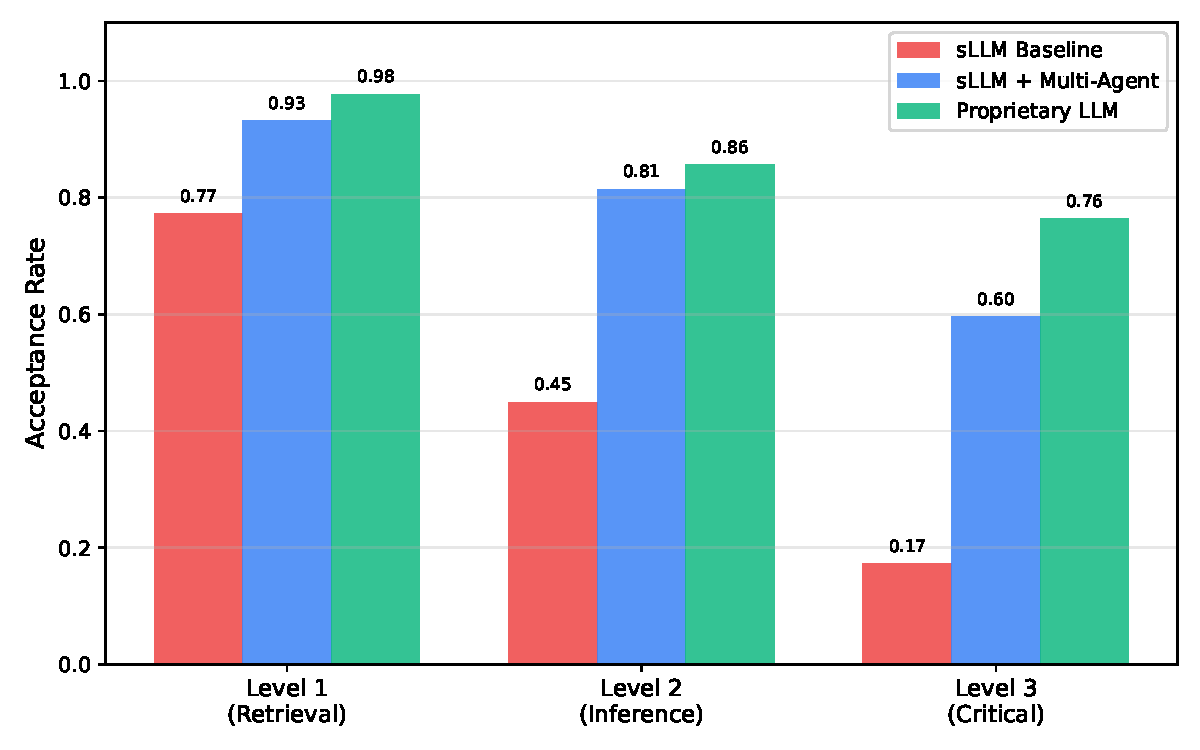
\includegraphics[width=0.85\textwidth]{figures/group_comparison.pdf}
\caption{So sánh chỉ số Acceptance trung bình giữa ba nhóm mô hình theo cấp độ nhận thức}
\label{fig:group_comparison}
\end{figure}

% [NEW]
Kết quả so sánh cho thấy ba phát hiện chính. Thứ nhất, ở Cấp 1 và Cấp 2, nhóm sLLM kết hợp đa tác tử đạt kết quả cạnh tranh sát sao với nhóm LLM thương mại. Cụ thể, Phi-4 kết hợp đa tác tử đạt Acceptance 0,9753 ở Cấp 1 và 0,9072 ở Cấp 2, trong khi Gemini 3 Flash đạt 0,9820 và 0,9280 tương ứng - chênh lệch không đáng kể. Thứ hai, ở Cấp 3, nhóm LLM thương mại vẫn duy trì ưu thế rõ rệt, đặc biệt ở chỉ số Distractor Quality, nơi Gemini 3 Flash đạt 0,8980 trong khi Gemma 3 12B IT kết hợp đa tác tử chỉ đạt 0,6600. Thứ ba, khoảng cách chất lượng giữa nhóm sLLM cơ bản và hai nhóm còn lại là rất lớn ở Cấp 2 và Cấp 3, khẳng định vai trò thiết yếu của kiến trúc đa tác tử hoặc năng lực mô hình lớn trong việc sinh câu hỏi tư duy bậc cao.

% [NEW]
\section{Kết quả OCR}

% [NEW]
% [MODIFY]: Cap nhat mo ta section OCR bao gom ca VLM va LLM thuong mai
Phần này đánh giá khả năng nhận dạng ký tự quang học (OCR) của bảy mô hình: bốn mô hình thị giác-ngôn ngữ quy mô nhỏ chuyên dụng và ba mô hình ngôn ngữ lớn thương mại đa phương thức, trên hai điều kiện: ảnh sạch (chất lượng cao, không nhiễu) và ảnh nhiễu (đã qua tăng cường dữ liệu mô phỏng điều kiện thực tế). Hai chỉ số đánh giá được sử dụng là Tỷ lệ lỗi ký tự (CER - Character Error Rate) và Tỷ lệ lỗi từ (WER - Word Error Rate), trong đó giá trị càng thấp thể hiện chất lượng OCR càng tốt.

% [NEW]
\subsection{Kết quả trên ảnh sạch}

% [NEW]
Bảng~\ref{tab:ocr_clean} trình bày kết quả OCR trên tập ảnh sạch, nơi văn bản được chụp trong điều kiện lý tưởng với độ phân giải cao và không có nhiễu.

% [MODIFY]: Gop du lieu LLM thuong mai vao bang OCR anh sach
\begin{table}[htbp]
\centering
\caption{Kết quả OCR trên ảnh sạch}
\label{tab:ocr_clean}
\begin{tabular}{lcc}
\toprule
\textbf{Mô hình} & \textbf{CER} & \textbf{WER} \\
\midrule
DeepSeek OCR 2 & 0,0681 & 0,0948 \\
DotOCR 1.5 & 0,0075 & 0,0172 \\
MinerU 2.5 & 0,0252 & 0,0427 \\
PaddleOCR VL 1.5 & 0,0113 & 0,0232 \\
\midrule
Gemini 3 Flash & 0,0084 & 0,0141 \\
GPT-5 Mini & 0,0150 & 0,0209 \\
Claude Haiku 4.5 & 0,0238 & 0,0337 \\
\bottomrule
\end{tabular}
\end{table}

% [MODIFY]: Viet lai nhan xet anh sach bao gom ca VLM va LLM thuong mai
Trên ảnh sạch, DotOCR 1.5 đạt kết quả tốt nhất trong nhóm mô hình nhỏ gọn với CER chỉ 0,0075 và WER 0,0172, tương đương với hơn 99\% ký tự được nhận dạng chính xác. Gemini 3 Flash đạt kết quả gần tương đương với CER 0,0084 và WER 0,0141, là mô hình thương mại có hiệu suất OCR tốt nhất. PaddleOCR VL 1.5 xếp thứ ba với CER 0,0113. Trong nhóm thương mại, GPT-5 Mini (CER 0,0150) và Claude Haiku 4.5 (CER 0,0238) đều đạt kết quả tốt, trong khi DeepSeek OCR 2 có CER cao nhất (0,0681). Nhìn chung, trên ảnh sạch, khoảng cách giữa các mô hình nhỏ gọn tốt nhất và mô hình thương mại là không đáng kể.

% [NEW]
\subsection{Kết quả trên ảnh nhiễu}

% [NEW]
Bảng~\ref{tab:ocr_augmented} trình bày kết quả OCR trên tập ảnh đã qua tăng cường dữ liệu (data augmentation), mô phỏng các điều kiện chụp ảnh thực tế như nghiêng, mờ, nhiễu hạt và thay đổi ánh sáng.

% [MODIFY]: Gop du lieu LLM thuong mai vao bang OCR anh nhieu
\begin{table}[htbp]
\centering
\caption{Kết quả OCR trên ảnh nhiễu (đã tăng cường dữ liệu)}
\label{tab:ocr_augmented}
\begin{tabular}{lcc}
\toprule
\textbf{Mô hình} & \textbf{CER} & \textbf{WER} \\
\midrule
DeepSeek OCR 2 & 0,1158 & 0,1579 \\
DotOCR 1.5 & 0,1467 & 0,1771 \\
MinerU 2.5 & 0,1079 & 0,2769 \\
PaddleOCR VL 1.5 & 0,1143 & 0,1473 \\
\midrule
Gemini 3 Flash & 0,0204 & 0,0326 \\
GPT-5 Mini & 0,0269 & 0,0409 \\
Claude Haiku 4.5 & 0,1799 & 0,1932 \\
\bottomrule
\end{tabular}
\end{table}

% [MODIFY]: Viet lai nhan xet anh nhieu bao gom ca VLM va LLM thuong mai
Kết quả trên ảnh nhiễu cho thấy sự phân hóa rõ rệt giữa hai nhóm mô hình. Gemini 3 Flash thể hiện khả năng kháng nhiễu vượt trội nhất: CER chỉ tăng từ 0,0084 lên 0,0204 (tăng 2,4 lần), trong khi các mô hình nhỏ gọn tốt nhất tăng từ 10 đến 20 lần. GPT-5 Mini cũng duy trì hiệu suất ổn định với CER 0,0269 trên ảnh nhiễu. Hai mô hình thương mại này vượt trội hẳn so với toàn bộ nhóm mô hình nhỏ gọn trong điều kiện nhiễu.

Trong nhóm mô hình nhỏ gọn, MinerU 2.5 đạt CER thấp nhất (0,1079) nhưng lại có WER cao nhất (0,2769), cho thấy mô hình này nhận dạng ký tự tương đối tốt nhưng gặp khó khăn trong việc ghép từ chính xác. PaddleOCR VL 1.5 thể hiện sự cân bằng tốt nhất với cả CER (0,1143) và WER (0,1473) đều ở mức trung bình thấp. DotOCR 1.5, mô hình tốt nhất trên ảnh sạch, lại chịu mức suy giảm lớn nhất: CER tăng gần 20 lần từ 0,0075 lên 0,1467.

Đáng chú ý, Claude Haiku 4.5 là ngoại lệ trong nhóm thương mại: CER tăng từ 0,0238 lên 0,1799 (tăng 7,6 lần), ngang mức suy giảm của các mô hình nhỏ gọn. Kết quả này cho thấy khả năng kháng nhiễu không hoàn toàn tương quan với quy mô mô hình, mà phụ thuộc vào chiến lược huấn luyện và dữ liệu tiền xử lý của từng kiến trúc.

% [NEW]
Hình~\ref{fig:ocr_comparison} so sánh trực quan hiệu suất OCR giữa hai điều kiện ảnh, cho thấy rõ mức độ suy giảm khi chuyển từ ảnh sạch sang ảnh nhiễu.

% [NEW]
\begin{figure}[htbp]
\centering
% [MODIFY]: Thay placeholder bang bieu do thuc te bao gom ca VLM va LLM thuong mai
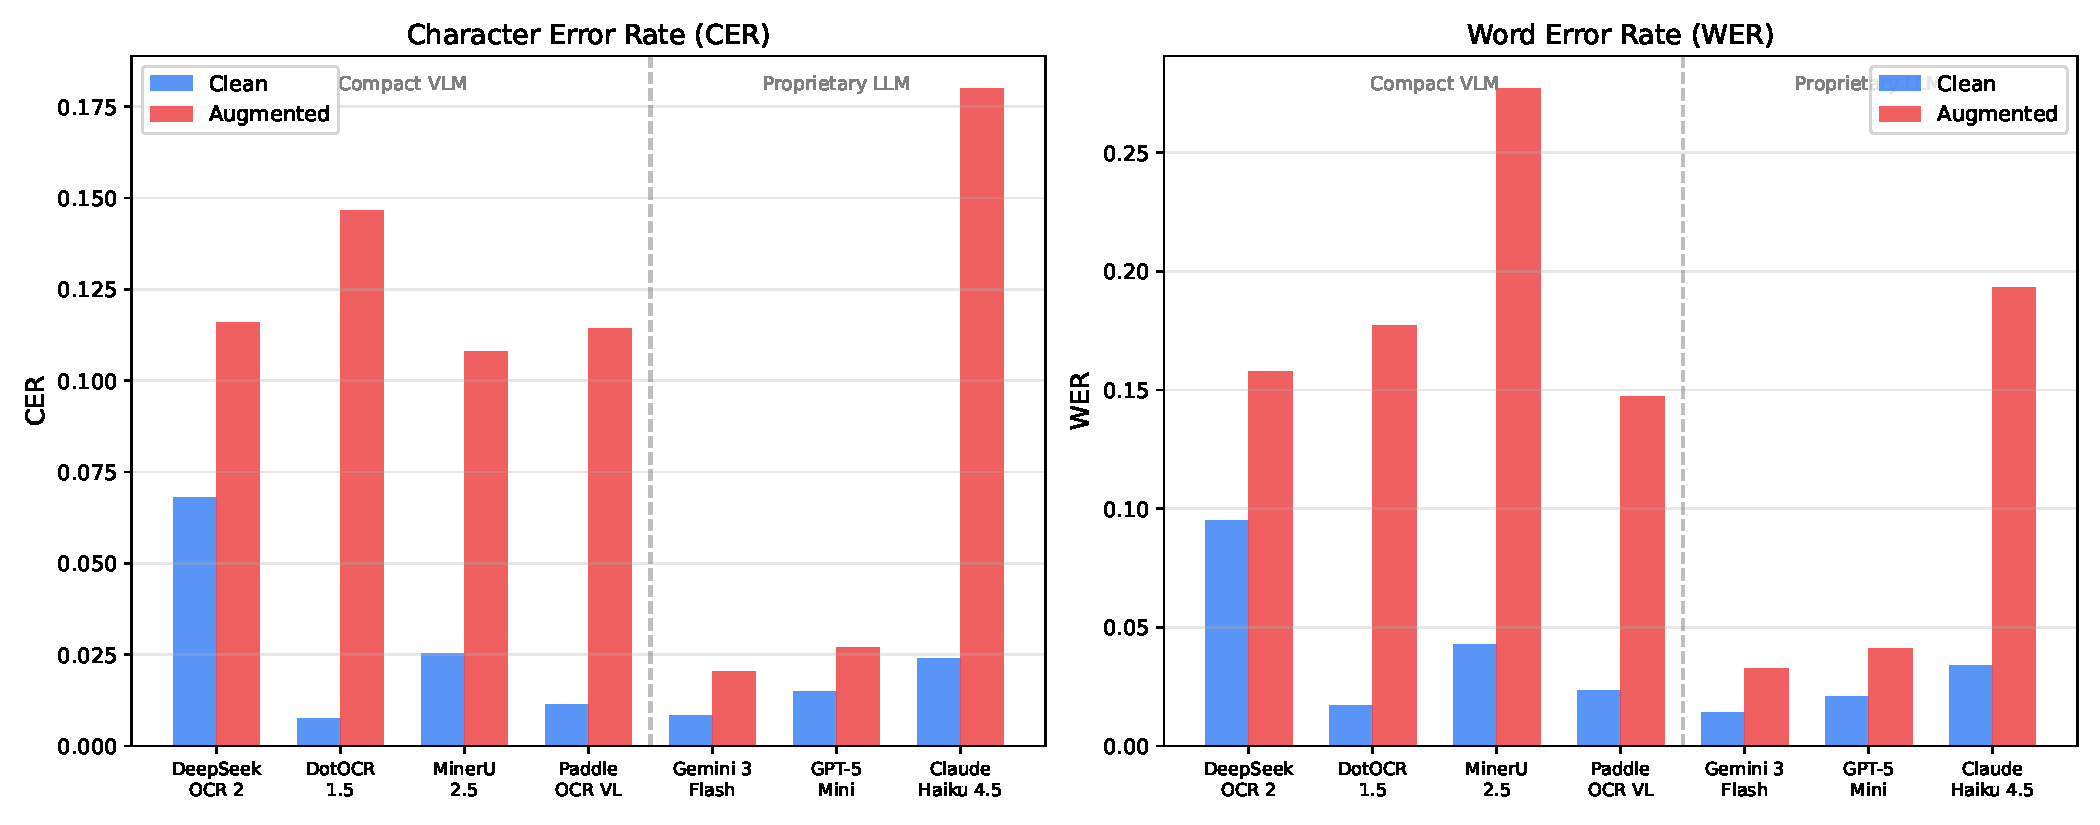
\includegraphics[width=\textwidth]{figures/ocr_comparison.pdf}
\caption{So sánh hiệu suất OCR giữa ảnh sạch và ảnh nhiễu}
\label{fig:ocr_comparison}
\end{figure}

% [MODIFY]: Xoa section 5.4.3 rieng biet vi du lieu da gop vao bang chinh

% [NEW]
\section{Phân tích chi phí}

% [NEW]
Bên cạnh chất lượng, chi phí sử dụng API là một yếu tố quan trọng trong việc lựa chọn giải pháp triển khai thực tế. Bảng~\ref{tab:cost} trình bày chi phí trung bình cho việc xử lý 100 đoạn văn mẫu (tương đương tối đa 1.500 câu hỏi) của từng cấu hình mô hình, được theo dõi thông qua OpenRouter API.

% [NEW]
\begin{table}[htbp]
\centering
\caption{Chi phí sử dụng API cho 100 đoạn văn mẫu (USD)}
\label{tab:cost}
\begin{tabular}{llr}
\toprule
\textbf{Nhóm} & \textbf{Mô hình} & \textbf{Chi phí (USD)} \\
\midrule
\multirow{5}{*}{sLLM cơ bản} & Gemma 3 12B IT & \$0,02 \\
& Qwen3 8B & \$0,01 \\
& Phi-4 & \$0,02 \\
& Nemotron Nano 9B v2 & \$0,02 \\
% [MODIFIED]: Chuan hoa ten mo hinh ve Llama 3.1 8B Instruct de dong bo voi bang ket qua G-Eval, thu muc outputs va cac phan mo ta con lai cua bao cao.
& Llama 3.1 8B Instruct & \$0,04 \\
\midrule
\multirow{5}{*}{sLLM + đa tác tử} & Gemma 3 12B IT & \$0,21 \\
& Qwen3 8B & \$0,18 \\
& Phi-4 & \$0,19 \\
& Nemotron Nano 9B v2 & \$0,30 \\
& Llama 3.1 8B Instruct & \$0,47 \\
\midrule
\multirow{3}{*}{LLM thương mại} & Gemini 3 Flash & \$0,46 \\
& GPT-5 Mini & \$0,26 \\
& Claude Haiku 4.5 & \$0,80 \\
\bottomrule
\end{tabular}
\end{table}

% [NEW]
Hình~\ref{fig:cost_quality} trình bày biểu đồ phân tích mối quan hệ giữa chi phí và chất lượng (đo bằng Acceptance trung bình trên ba cấp độ) cho từng cấu hình mô hình.

% [NEW]
\begin{figure}[htbp]
\centering
% [MODIFY]: Thay placeholder bang bieu do thuc te
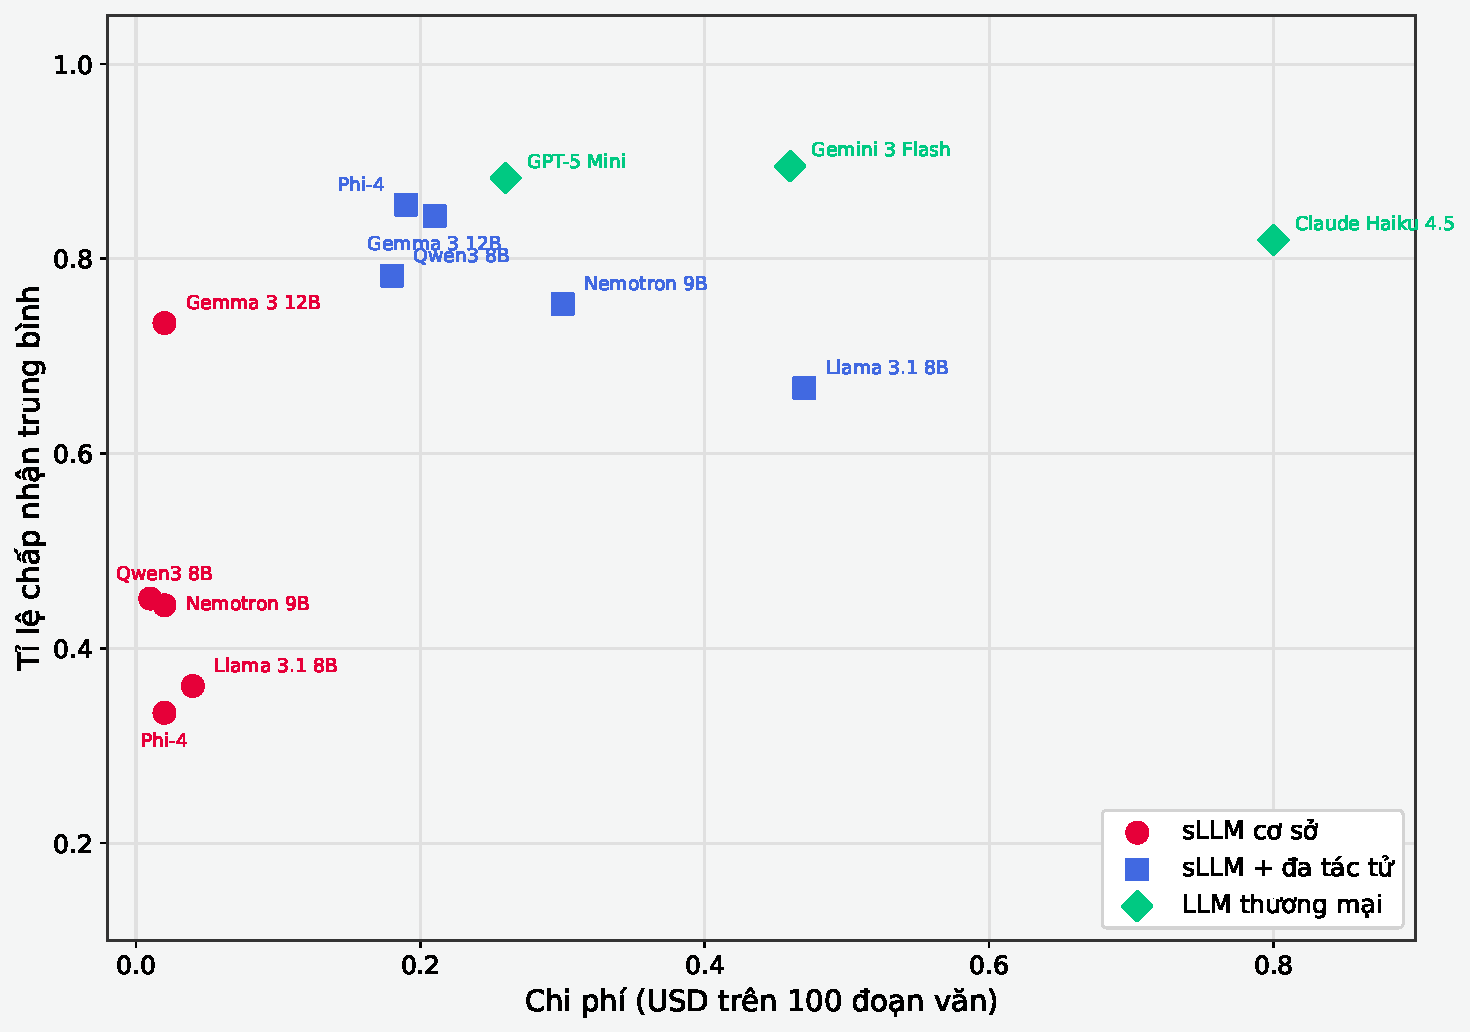
\includegraphics[width=0.85\textwidth]{figures/cost_quality.pdf}
\caption{Phân tích mối quan hệ giữa chi phí và chất lượng sinh câu hỏi}
\label{fig:cost_quality}
\end{figure}

% [NEW]
Phân tích chi phí cho thấy ba điểm đáng chú ý. Thứ nhất, nhóm sLLM cơ bản có chi phí cực thấp (từ \$0,01 đến \$0,04 cho 100 đoạn văn), tuy nhiên chất lượng ở Cấp 2 và Cấp 3 không đáp ứng được yêu cầu thực tế. Thứ hai, hệ thống đa tác tử làm tăng chi phí khoảng 10 đến 20 lần so với sLLM cơ bản (ví dụ: Gemma từ \$0,02 lên \$0,21, Qwen3 từ \$0,01 lên \$0,18), nhưng mức cải thiện chất lượng thu được là vượt trội - đặc biệt ở Cấp 2 và Cấp 3 - tạo ra tỷ suất lợi ích trên chi phí rất cao. Thứ ba, so với nhóm LLM thương mại, cấu hình Gemma 3 12B IT kết hợp đa tác tử nổi lên như lựa chọn tối ưu theo biên Pareto: chỉ với \$0,21 (bằng 45,7\% chi phí của Gemini 3 Flash và 26,3\% chi phí của Claude Haiku 4.5), cấu hình này đạt chất lượng cạnh tranh ở Cấp 1 và Cấp 2, đồng thời duy trì kết quả chấp nhận được ở Cấp 3.

% [NEW]
\section{Thảo luận}

% [NEW]
Từ kết quả thực nghiệm được trình bày ở các phần trên, nghiên cứu rút ra sáu nhận định chính.

% [NEW]
\textbf{Hệ thống đa tác tử đóng vai trò ``bộ khuếch đại chất lượng'' cho sLLM.} Kết quả cho thấy kiến trúc đa tác tử không chỉ cải thiện chất lượng mà còn thể hiện một đặc tính quan trọng: các mô hình có kết quả cơ bản yếu nhất lại hưởng lợi nhiều nhất. Phi-4, với Distractor Quality ở Cấp 1 chỉ đạt 0,4860 khi hoạt động đơn lẻ, đã tăng lên 0,9407 khi kết hợp đa tác tử - mức cải thiện 93,6\%. Llama 3.1 8B Instruct ghi nhận cải thiện Acceptance ở Cấp 3 hơn 21 lần. Điều này gợi ý rằng hệ thống đa tác tử hoạt động hiệu quả nhất khi mô hình nền có năng lực tiềm ẩn chưa được khai thác đầy đủ trong chế độ hoạt động đơn lẻ.

% [NEW]
\textbf{Tác tử Phân loại hoạt động hiệu quả nhờ kỹ thuật ánh xạ mã định danh tạm thời.} Chỉ số Alignment đạt gần hoặc bằng 1,0 ở Cấp 2 và Cấp 3 cho hầu hết các mô hình trong nhóm đa tác tử (Qwen3 8B và Phi-4 đạt 1,0000 ở Cấp 3) chứng tỏ kỹ thuật ánh xạ mã định danh tạm thời - thay thế nhãn cấp độ bằng các ký hiệu trung tính để chống thiên lệch vị trí - hoạt động rất tốt. Đây là một trong những đóng góp kỹ thuật quan trọng của nghiên cứu, giúp đảm bảo tính khách quan trong quá trình phân loại câu hỏi theo thang nhận thức Bloom.

% [NEW]
\textbf{Tác tử Học sinh đóng vai trò lọc câu hỏi mơ hồ.} Bằng cách mô phỏng quá trình trả lời của học sinh, tác tử này giúp phát hiện các câu hỏi có đề bài thiếu rõ ràng, phương án nhiễu quá dễ loại trừ, hoặc đáp án không phân biệt rõ với các phương án sai. Cơ chế phản hồi từ Tác tử Học sinh đến Tác tử Hiệu chỉnh tạo thành vòng lặp cải tiến liên tục, giúp nâng cao chất lượng câu hỏi qua nhiều vòng.

% [NEW]
\textbf{Biên Pareto: Gemma 3 12B IT kết hợp đa tác tử là lựa chọn giá trị tối ưu.} Khi xem xét đồng thời chi phí và chất lượng, cấu hình Gemma 3 12B IT với hệ thống đa tác tử nổi lên là điểm tối ưu trên biên Pareto. Với chi phí chỉ \$0,21 cho 100 đoạn văn, cấu hình này đạt Acceptance 0,9580 (Cấp 1), 0,8380 (Cấp 2) và 0,7360 (Cấp 3), vượt trội so với Claude Haiku 4.5 (\$0,80) ở cả ba cấp độ và cạnh tranh sát sao với Gemini 3 Flash (\$0,46) ở Cấp 1 và Cấp 2.

% [NEW]
% [MODIFY]: Cap nhat nhan dinh OCR bao gom ca LLM thuong mai
\textbf{OCR: mô hình nhỏ gọn gặp khó khăn với ảnh nhiễu, mô hình thương mại phân hóa rõ rệt.} Kết quả OCR cho thấy dù các mô hình nhỏ gọn hoạt động tốt trên ảnh sạch (DotOCR 1.5 đạt CER 0,0075), hiệu suất suy giảm đáng kể trên ảnh nhiễu (CER tăng lên 0,1079-0,1467). Trong khi đó, Gemini 3 Flash và GPT-5 Mini duy trì hiệu suất ổn định trên ảnh nhiễu (CER lần lượt 0,0204 và 0,0269), nhưng Claude Haiku 4.5 lại chịu mức suy giảm tương đương nhóm mô hình nhỏ gọn (CER 0,1799). Phát hiện này nhấn mạnh rằng khả năng kháng nhiễu phụ thuộc vào chiến lược huấn luyện chứ không hoàn toàn vào quy mô mô hình, đồng thời nhấn mạnh tầm quan trọng của bước tiền xử lý ảnh trong đường ống xử lý thực tế.

% [NEW]
\textbf{Hạn chế của phương pháp đánh giá LLM-as-a-Judge.} Toàn bộ kết quả đánh giá trong nghiên cứu này được thực hiện bằng phương pháp G-Eval, sử dụng mô hình ngôn ngữ lớn làm người đánh giá tự động. Mặc dù phương pháp này cho phép đánh giá quy mô lớn với chi phí thấp và tính nhất quán cao, nó vẫn thiếu sự đối chiếu với đánh giá của con người - tiêu chuẩn vàng trong đánh giá chất lượng giáo dục. Các nghiên cứu trước đã chỉ ra rằng LLM-as-a-Judge có thể mắc các thiên lệch như ưu tiên câu trả lời dài hơn hoặc thiên vị đầu ra của chính mình. Do đó, các kết quả định lượng trong nghiên cứu này cần được diễn giải với sự thận trọng phù hợp.

% [NEW]
\section{Hạn chế và hướng phát triển}

% [NEW]
\subsection{Hạn chế}

% [NEW]
Nghiên cứu này có một số hạn chế cần được ghi nhận. Thứ nhất, toàn bộ thực nghiệm chỉ được tiến hành trên một bộ dữ liệu duy nhất (RACE-High) với 100 đoạn văn mẫu, chưa đủ để khẳng định tính tổng quát của kết quả trên các miền dữ liệu khác như khoa học, y tế hay pháp luật. Thứ hai, dữ liệu đầu vào hoàn toàn bằng tiếng Anh, chưa kiểm chứng hiệu quả của hệ thống trên các ngôn ngữ khác, đặc biệt là tiếng Việt - ngôn ngữ mục tiêu ứng dụng của hệ thống Openlet. Thứ ba, nghiên cứu thiếu đánh giá bởi con người để đối chiếu với kết quả G-Eval, khiến không thể xác định chính xác mức độ tương quan giữa đánh giá tự động và nhận định của giáo viên thực tế. Thứ tư, chi phí API có thể biến động theo thời gian do chính sách giá của các nhà cung cấp, làm giảm tính ổn định của phân tích chi phí-hiệu quả.

% [NEW]
\subsection{Hướng phát triển}

% [NEW]
Dựa trên các hạn chế đã xác định, nghiên cứu đề xuất năm hướng phát triển chính:

% [NEW]
\begin{enumerate}
    \item \textbf{Hỗ trợ đa ngôn ngữ, ưu tiên tiếng Việt:} Mở rộng hệ thống để xử lý văn bản tiếng Việt, bao gồm việc xây dựng bộ dữ liệu đánh giá tiếng Việt và điều chỉnh các tác tử cho phù hợp với đặc thù ngôn ngữ (thanh điệu, từ ghép, cấu trúc câu).

    \item \textbf{Đánh giá bởi con người:} Tiến hành đánh giá bởi giáo viên và chuyên gia giáo dục trên một mẫu đại diện các câu hỏi sinh ra, nhằm xác định hệ số tương quan giữa G-Eval và đánh giá con người, đồng thời phát hiện các loại lỗi mà đánh giá tự động có thể bỏ sót.

    \item \textbf{Tinh chỉnh sLLM chuyên biệt:} Sử dụng dữ liệu câu hỏi chất lượng cao được sinh ra bởi hệ thống đa tác tử (đặc biệt từ cấu hình Gemma kết hợp đa tác tử) làm dữ liệu huấn luyện để tinh chỉnh (fine-tuning) các sLLM, hướng tới việc giảm nhu cầu sử dụng đa tác tử trong giai đoạn sản xuất.

    \item \textbf{Tích hợp hệ thống quản lý học tập (LMS):} Phát triển giao diện lập trình ứng dụng (API) và các bộ kết nối (connector) để tích hợp hệ thống Openlet với các nền tảng LMS phổ biến như Moodle, Canvas và Google Classroom, cho phép giáo viên sử dụng công cụ sinh câu hỏi trực tiếp trong quy trình giảng dạy.

    \item \textbf{Kiểm tra thích ứng dựa trên lý thuyết đáp ứng câu hỏi (IRT):} Kết hợp hệ thống sinh câu hỏi đa cấp độ với thuật toán kiểm tra thích ứng trên máy tính (Computerized Adaptive Testing - CAT), trong đó độ khó của câu hỏi tiếp theo được điều chỉnh tự động dựa trên năng lực ước lượng của người học, hướng tới trải nghiệm học tập cá nhân hóa.
\end{enumerate}
